\section{A Case for Parse Error Repair}
\label{sec:error-analysis}

We motivate \toolname by analyzing a dataset
comprising \emph{1,100,000 erroneous Python programs}
and their respective fixes.
%
This dataset was gathered from PythonTutor.com~\citep{Guo2013}
between the years 2017 and 2018, previously used in related
work~\citep{Endres2019, Cosman2020}.
%
Each program which throws an uncaught \python exception
is paired with the next program by the same user that does
not crash, under the assumption that the latter is the fixed
version of the former.
%
We discard pairs that are too different between buggy
and fixed versions, since these are usually unrelated
submissions or complete refactorings.
%
We also discard submissions that violate PythonTutor's
policies (\eg, those using forbidden libraries).
%
The resulting dataset contains usable program pairs,
representing students from dozens of universities
(PythonTutor has been used in many introductory
courses~\citep{Guo2013}) as well as non-traditional
novices.

\begin{figure}[t]
  \centering
  \begin{minipage}[c]{0.48\linewidth}
    \centering
    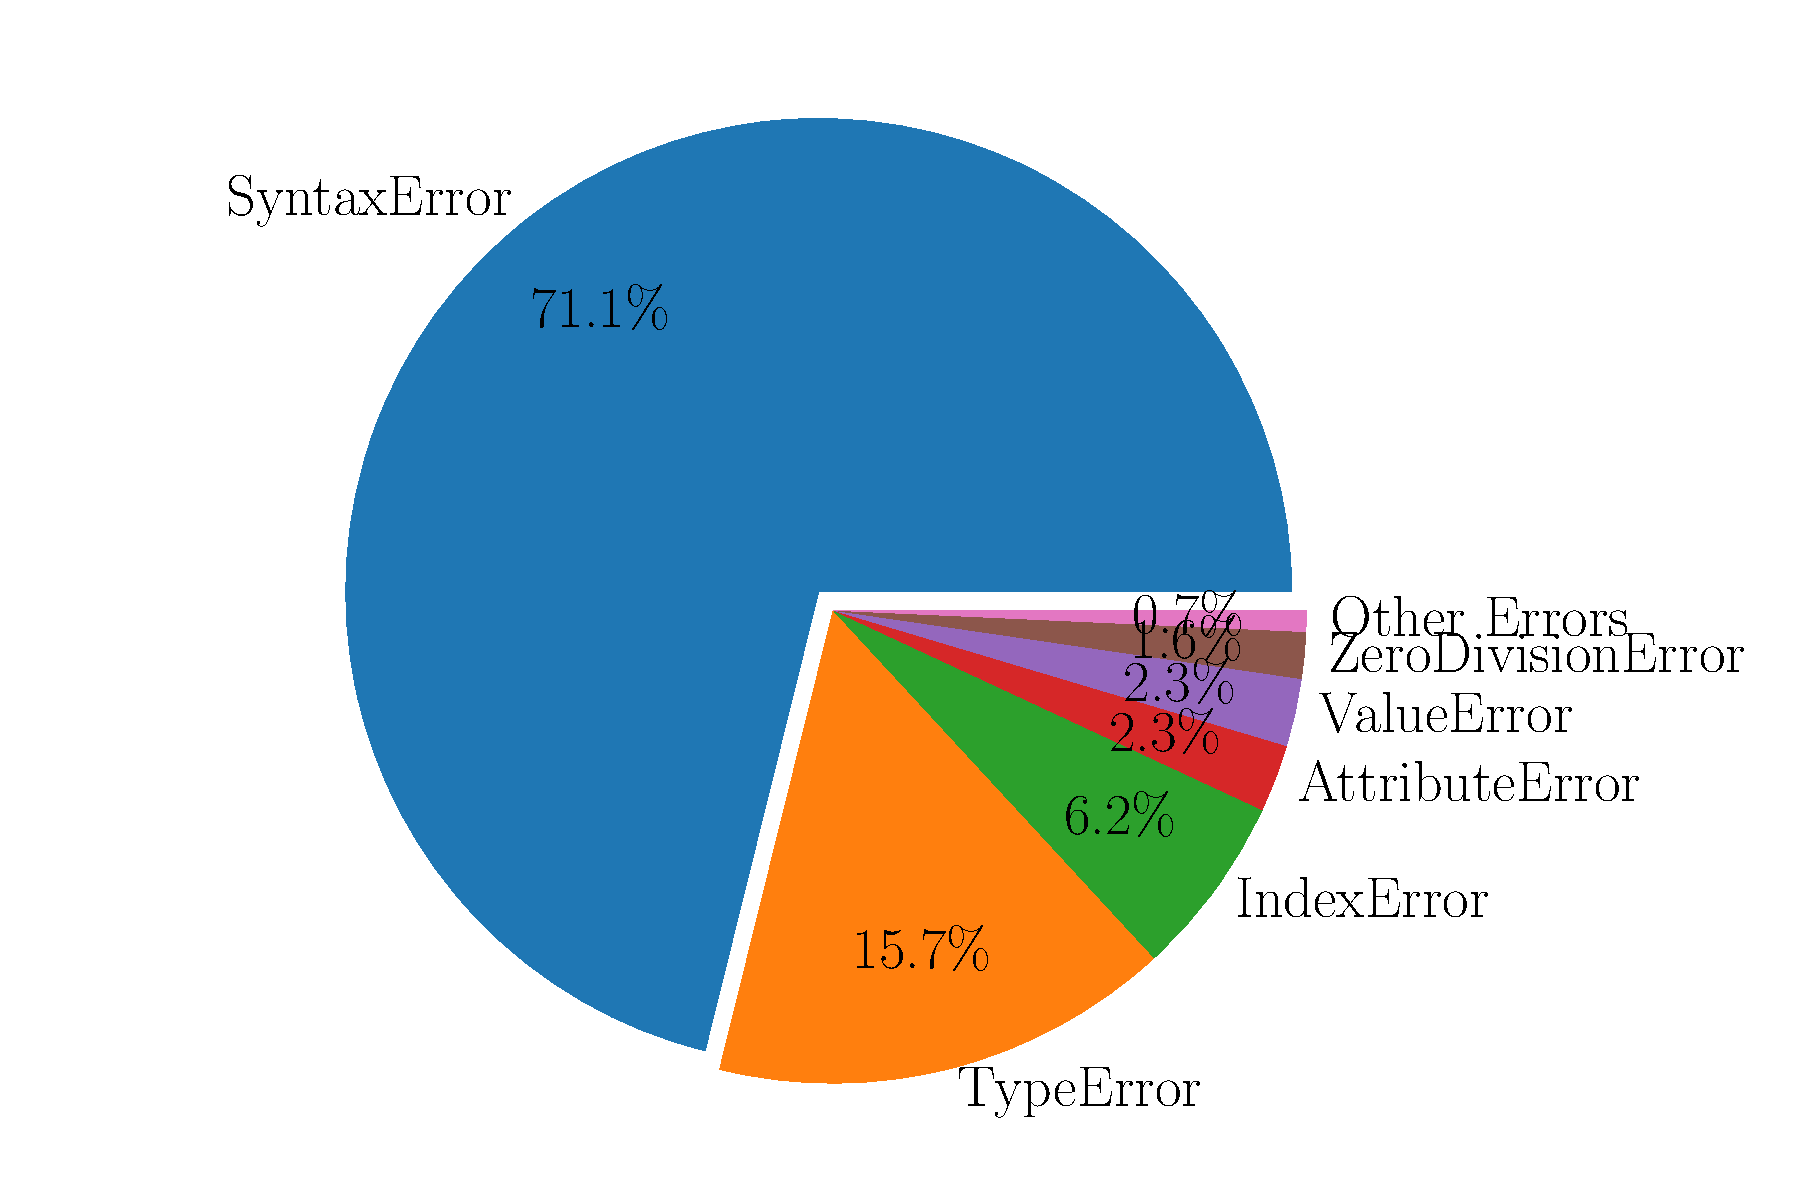
\includegraphics[width=\linewidth]{error-pie.pdf}
    \caption{The Python error type distribution.}
    \label{fig:error-statistics}
  \end{minipage}
  \hspace{0.02\linewidth}
  \begin{minipage}[c]{0.48\linewidth}
      \centering
      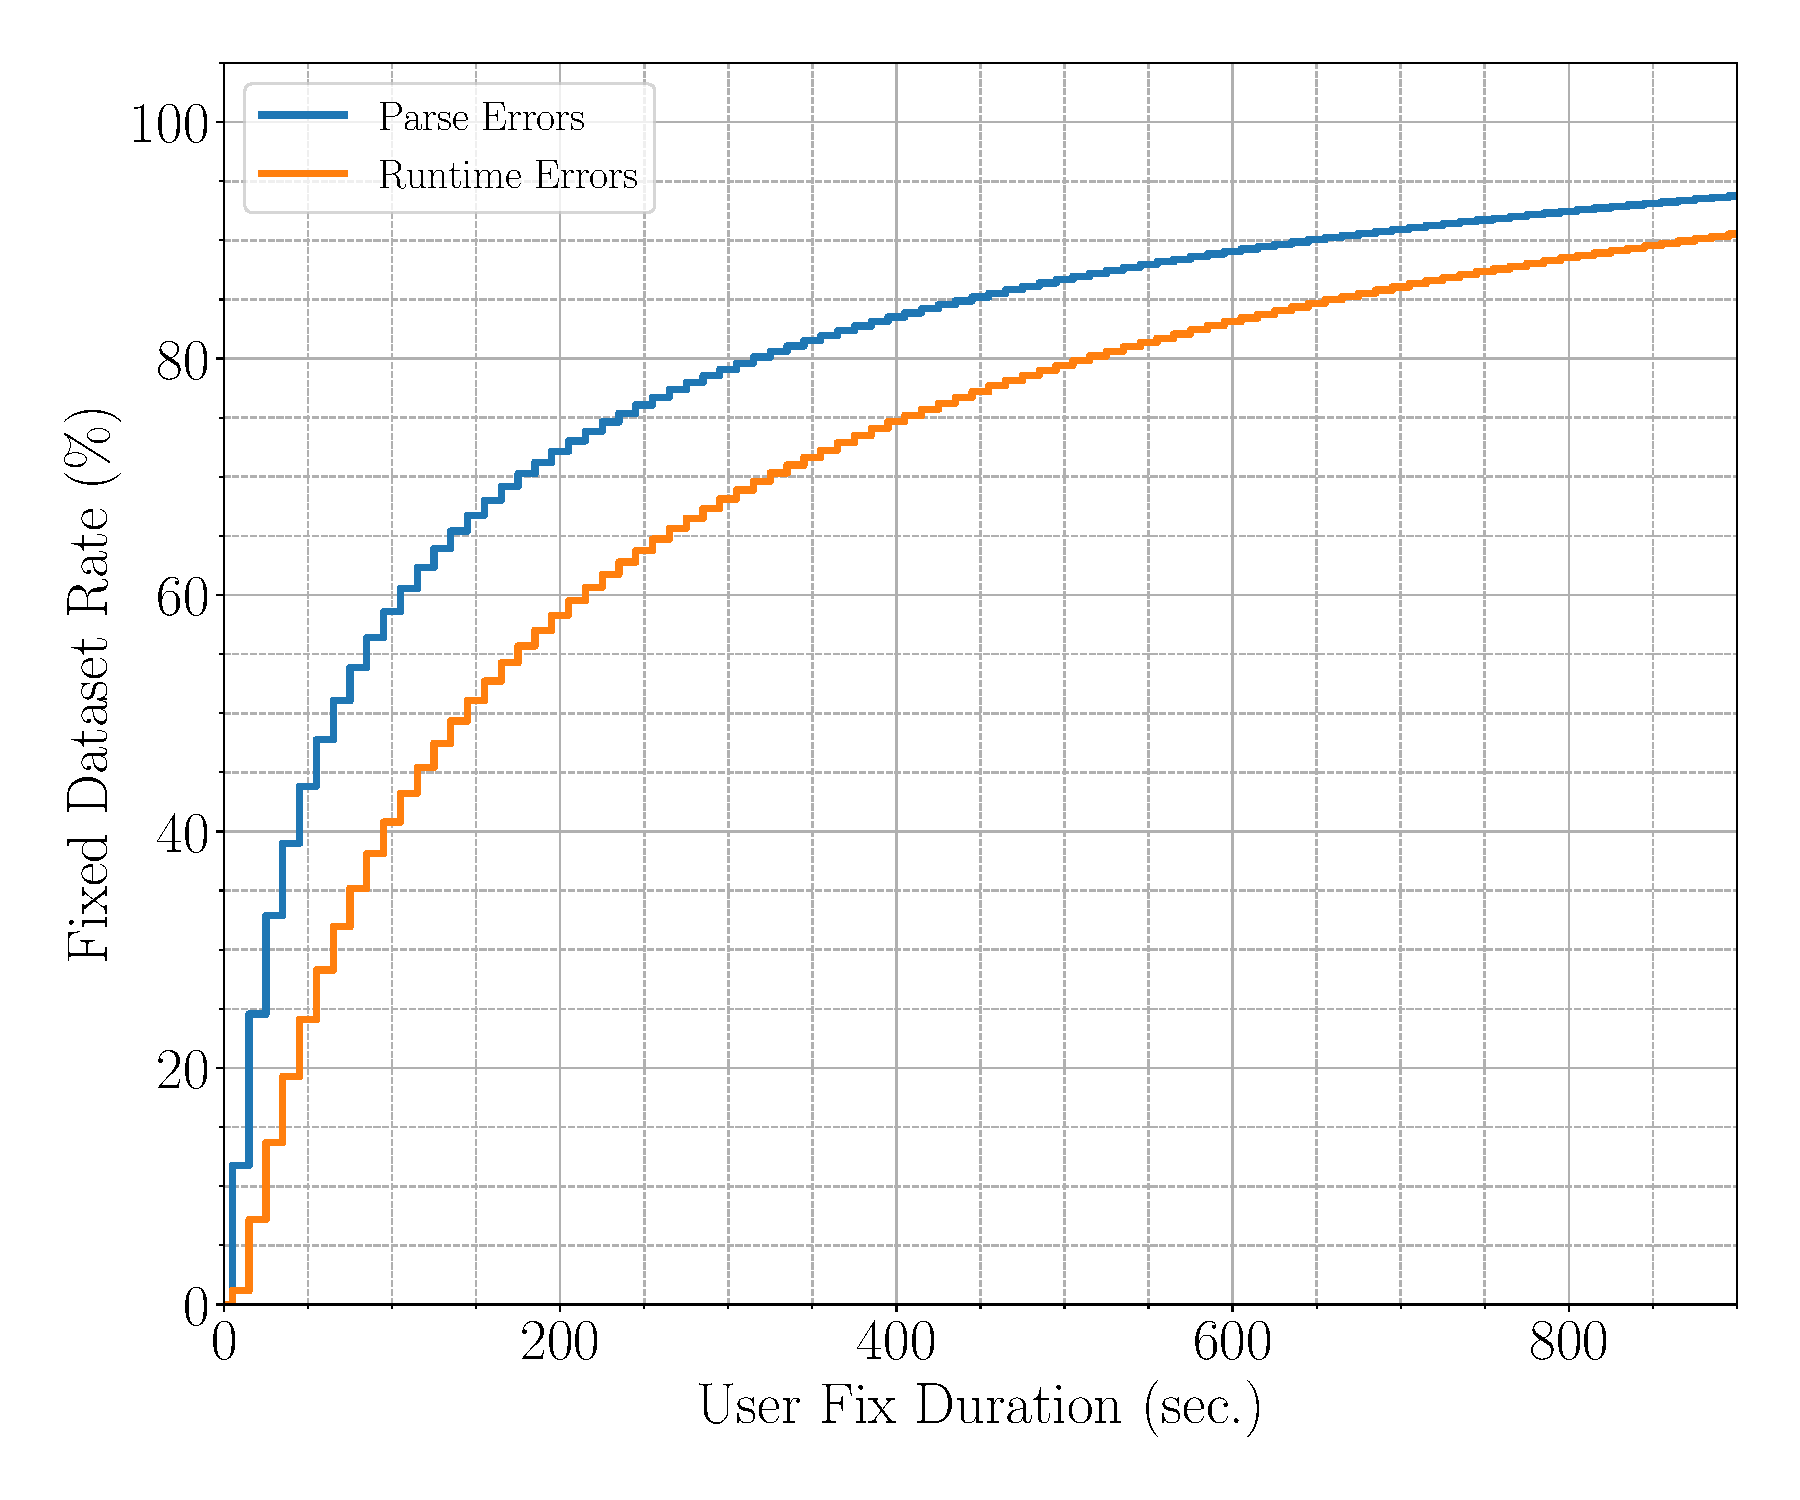
\includegraphics[width=\linewidth]{fixed-rate.pdf}
      \caption{The repair rates of the Python dataset.}
      \label{fig:repair-rate}
  \end{minipage}
\end{figure}

One might imagine that parse (or \emph{syntax}) errors are
usually easier to locate and repair than other algorithmic
or runtime errors \citep{Denny_2012}.
%
For example, the Python parser will immediately inform the programmer
about missing parentheses in function argument lists or for not having
the proper indents in a statement block.
%
However, as has also been shown in previous
work \citep{Ahadi_2018, Kummerfeld2003}, our
data confirms that programmers (especially novices)
deal with these kinds of errors regularly and
spend a considerable amount of time fixing them.

\mypara{Observation 1: Parse errors are very common}
%
\autoref{fig:error-statistics} presents the statistics
of the different types of errors that users encountered
in this dataset.
%
We observe that $77.4 \% $ of all faulty programs failed
with a syntax error, accounting for the vast majority of
the errors that (novice) programmers face with their
programs.
%
The second category is merely $13.6\%$ of the dataset and
represents Python type errors. This is a strong indication
that parse errors are a very common type of error.

\mypara{Observation 2: Parse errors take time to fix}
%
The web-based compiler that we used to generate this
dataset provides us with a \emph{server timestamp}.
%
The timestamp is associated with each program attempt
submission, erroneous or not. The \emph{repair time}
of an erroneous program is calculated by taking the
difference of the two timestamps of the erroneous and
fixed program.
%
This method can be an inaccurate metric of repair time,
as there are various reasons these timings may be exaggerated,
\eg users stepping away from the computer, internet lag \etc.
%
However, in aggregate, due to the large
dataset of program repairs these timings
can still be viewed as an appropriate metric
of the amount of time it took programmers to
repair their program errors.

\autoref{fig:repair-rate} shows the \emph{programmer repair rate},
\ie the dataset percentage that is repaired under a given amount of time.
%
It presents the repair rate for parse errors and the rest
of the error types, grouped together here as \emph{runtime} errors.
%
As expected, parse errors are fixed faster than the rest,
but \emph{not by a large difference}.
%
For example, we observe that within 2 minutes,
usually $46\%$ of the runtime errors are repaired, while
around $63\%$ of the syntax errors are.
%
Although, this is a considerable difference,
we observe that there is still a large number
of the ``simpler'' parse errors that required
more than 2 minutes to be fixed.

\begin{figure}[t]
  \centering
  \begin{minipage}[c]{0.48\linewidth}
    \centering
    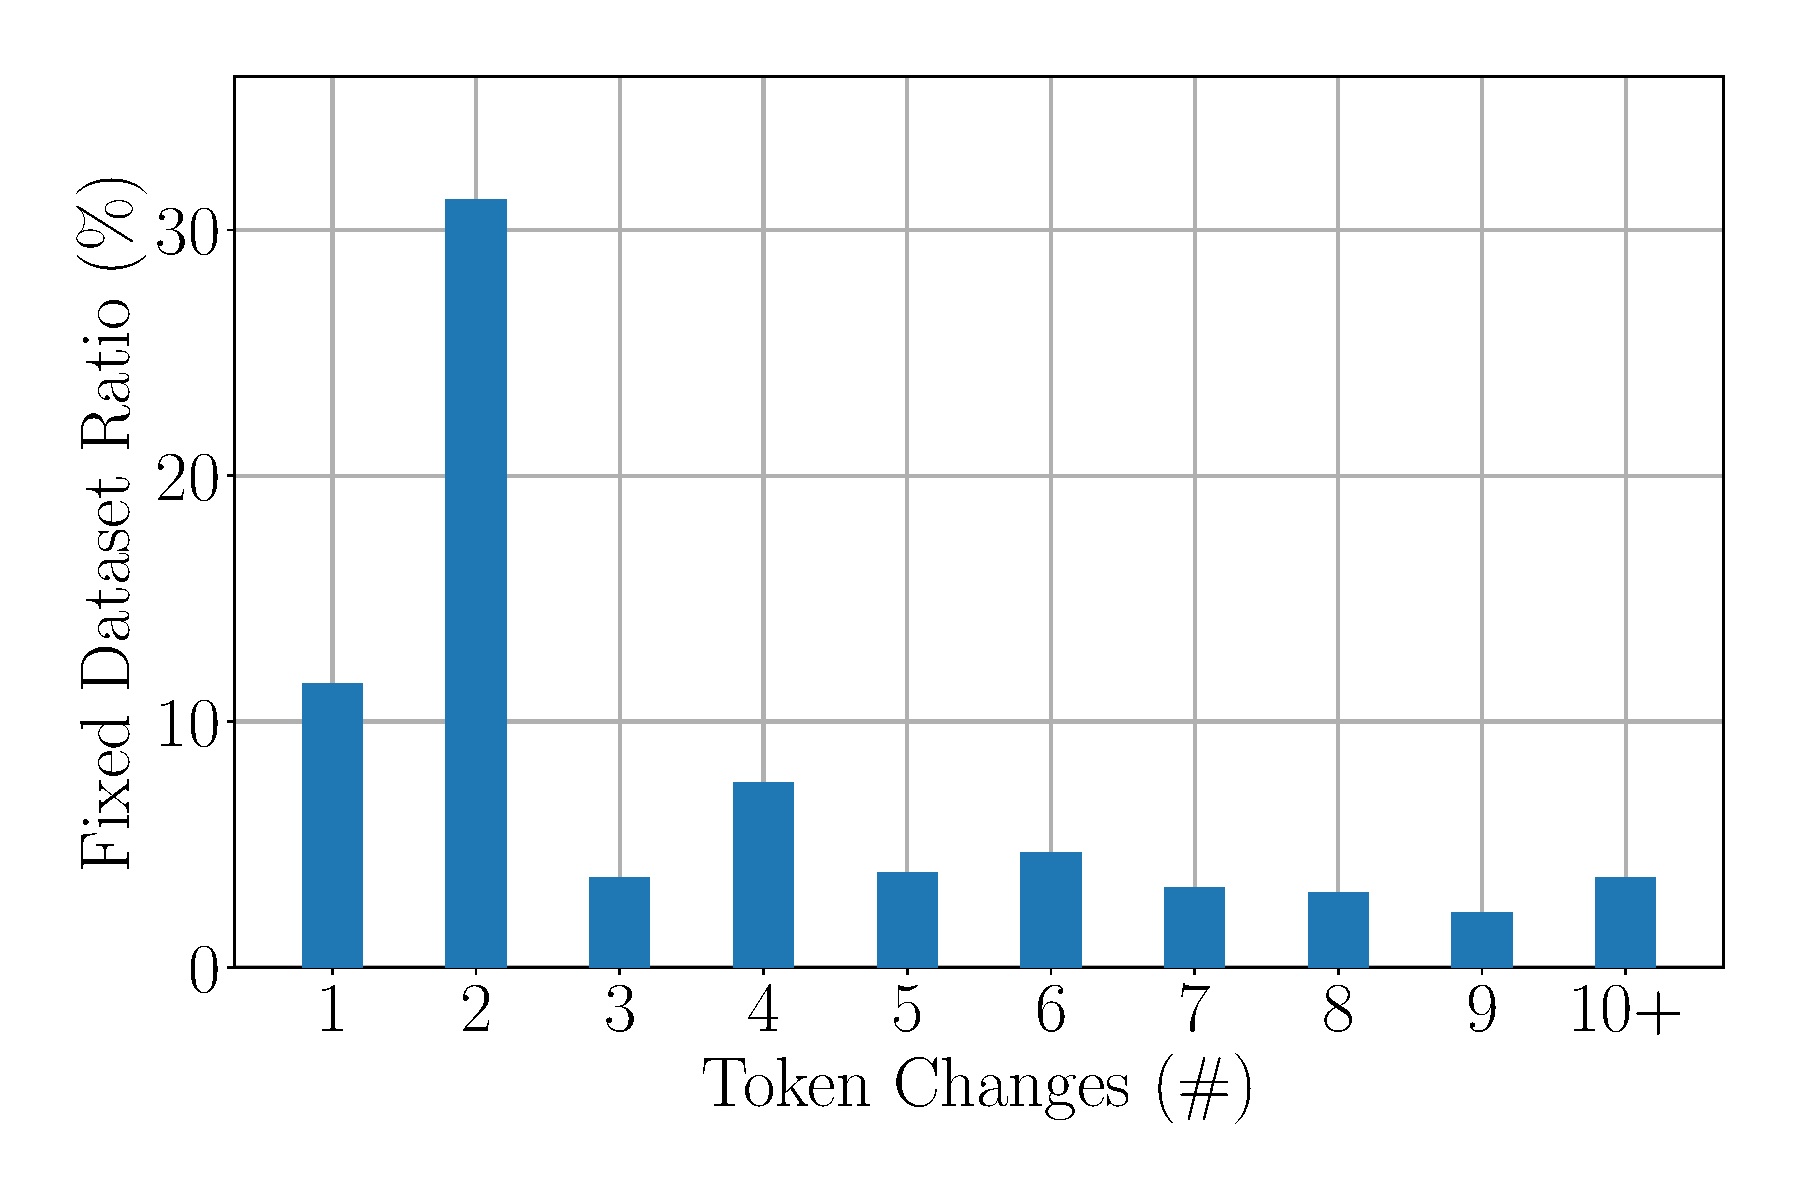
\includegraphics[width=\linewidth]{dataset-ratio-per-change.pdf}
    \caption{The Python dataset ratio that is fixed under the given number of
     token changes.}
    \label{fig:token-changes-ratio}
  \end{minipage}
  \hspace{0.02\linewidth}
  \begin{minipage}[c]{0.48\linewidth}
      \centering
      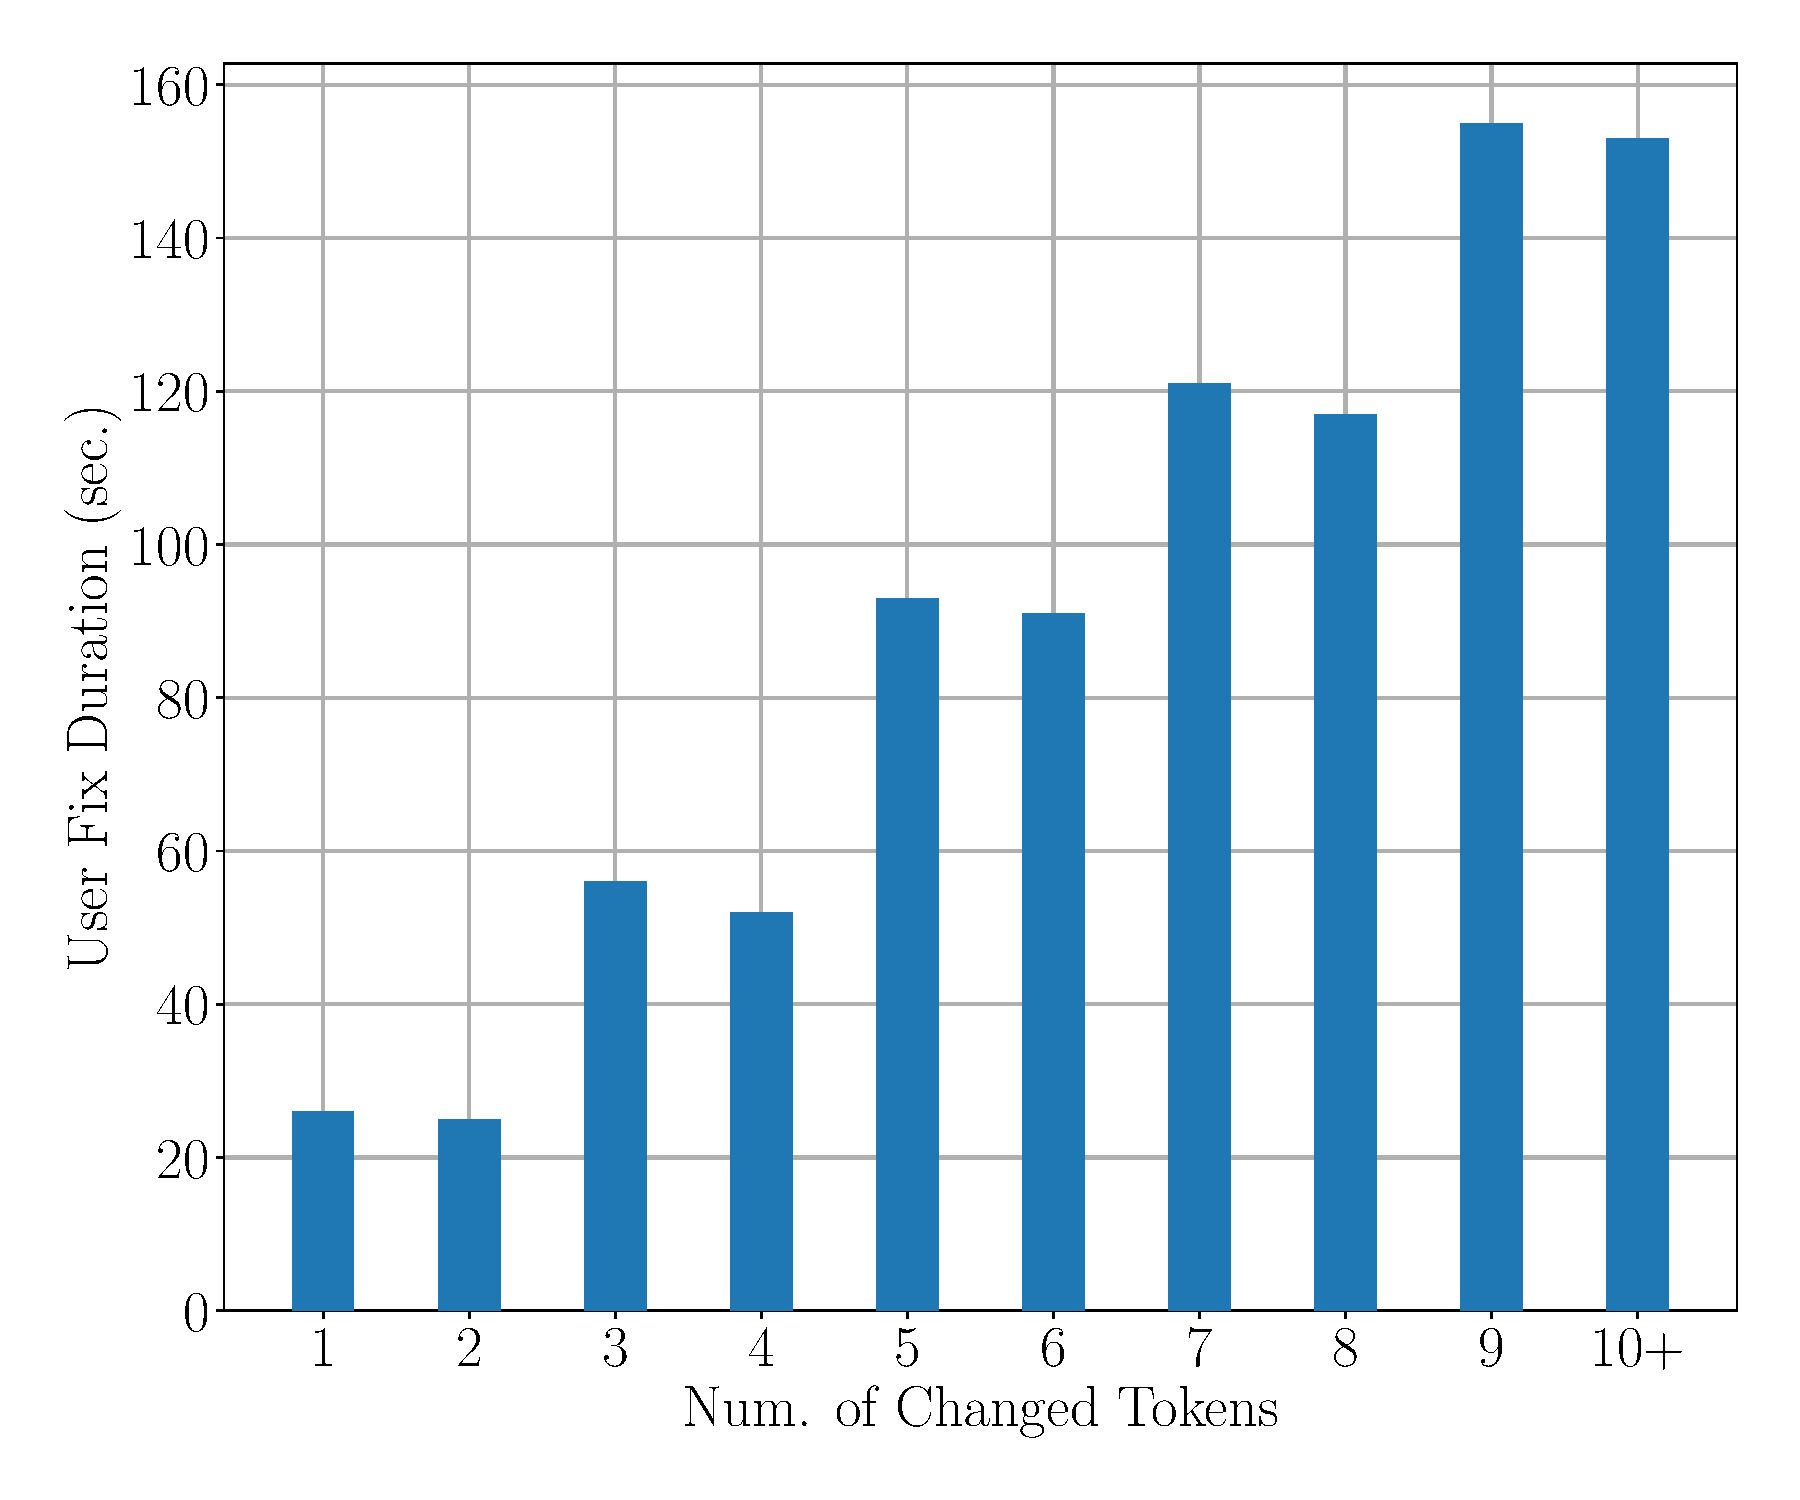
\includegraphics[width=\linewidth]{median-repair-times.pdf}
      \caption{The average time the user needed to fix the erroneous program
      for the needed token changes.}
      \label{fig:token-changes}
  \end{minipage}
\end{figure}

\mypara{Observation 3: Parse errors may need multiple edits to fix}
%
The average \emph{token-level changes} needed to fix a program with syntax
errors, \ie the number of changes in the lexed program token sequence, is
\emph{10.7 token changes}, while the \emph{median is 4}.
%
A variable rename or a different integer are not considered as changes
as they won't affect the syntax error fix.
%
As shown in \autoref{fig:token-changes-ratio}, $14.2\%$ of dataset
needs only 1 token change, $23.2\%$ needs 2 token changes, $7.0\%$
needs 3 and $9.0\%$ needs 4, \ie $53.4\%$ of the dataset needs at
most 4 token changes to be fixed.
%
While the majority of the syntax errors can be fixed with only a few
changes, the are still errors that need a lot of edits.
% It is also important to see how long it takes the users on average to make
% those changes.

\mypara{Observation 4: Parse errors with more edits take longer to fix}
%
\autoref{fig:token-changes} shows the average time that it takes a user to fix
all of their syntax errors per the number of token-level changes in their
programs. As expected, with an increasing number of token changes needed,
programmers need more time to implement those changes. Most importantly, even
for 1 or 2 token changes the average user spends \emph{26 and 25 sec}
respectively, which is still a considerable amount of time for such simple and
short fixes. The repair time jumps to \emph{56 sec} for three token changes.

\smallskip
These four observations indicate that, while simple syntax errors can usually be
easily and quickly fixed by programmers using the compiler error messages, they
can still struggle fixing programs that have more syntax errors.
%
Therefore, we can conclude that an automated tool that parses and repairs
such programs in only a few seconds could benefit many programmers.
